\chapter{Tests et analyse défauts fonctionnels ESD}
\label{chap:1}
\section{Contexte}

% What generates an ESD
Une décharge électrostatique est le résultat d'une accumulation de potentiel électrostatique, causée par induction électrique ou de la triboélectricité.
La charge triboélectrique se produit par transfert d'électrons lorsque deux objects sont mis en contact puis séparés.
Un objet se charge positivement et l'autre négativement.
Le signe de la charge dépend du matériau de l'objet.
La charge par induction se produit lorsque l'objet baigne dans un champs électrique, puis est soudainement mis à la masse.

% Electronic devices are exposed to ESD, in factories first
Les décharges électrostatiques sont un problème important pour les systèmes électroniques.
Des défaillances peuvent se produire pendant la fabrication ou pendant la vie du produit.
Pendant la fabrication, les circuits sont manipulés par des machines, ce qui cause des contacts répétés et éventuellement une accumulation de charges.
Il existe plusieurs standards de test pour garantir qu'un produit peut survivre aux étapes de fabrication.
Les testers HMM (Human Machine Model) et CDM (Charged Device Model) valident respectivement la robustesse vis-à-vis de la décharge d'un objet dans le produit, et la décharge du produit dans la masse.
Ces tests sont concus pour reproduire fidèlement les stress rencontrés dans l'environnement de fabrication.

% Electronic devices are exposed to ESD in the field
Des défaillances peuvent aussi apparaitre une fois le produit déployé sur le terrain.
Dans le cas de produits grand-public, elles peuvent être causées par la manipulation des objets par des humains chargés électriquement.
C'est le cas des téléphones portables et des caméras par exemple.
Dans l'environnement automobile, les contraintes sont encore plus fortes à cause d'autres phénomènes de génération de tribo-électricité.

% Hard-failure is one thing, soft-fail another
Il y a deux classes de défaillances dues aux ESD.
La casse matérielle est le premier type de défaillance.
Le composant est détruit après une décharge et doit être remplacé.
La perte de fonctionnalité est le second type, et se produit alors que le produit est alimenté et en fonctionnement normal.
La décharge perturbe une ou plusieurs fonctions, qui a besoin d'un délai pour récupérer.
Parfois, la fonction est bloquée et un rédemarrage manuel du produit est requis pour rétablir un fonctionnement normal.

\section{Méthodes de test ESD}

Pour reproduire les décharges électrostatiques dans un laboratoire, de multiples générateurs de test existent.
Le TLP (Transmission Line Pulser) est un des plus largement utilisés.
Il est employé dans une variété d'applications, pour la characterization de composants \cite{TLPforESDProtectionCz, TLPthroubleshooting}, l'investigation de défaillances \cite{tlp-application-1, tlp-application-2} et la correlation avec d'autre générateurs de test \cite{correlation-system-level-esd-tlp}.
Cette technique a été inventée par T. Maloney et N. Nakamura \cite{TLP}.
Elle est en cours de standardisation avec ANSI/ESD STM 5.5.1-2016 \cite{tlp-standard}.
Ce type de générateur a été longuement étudié dans les thèses de N. Monnereau \cite{phd-monnereau} et N. Lacrampe \cite{phd-lacrampe}.

% Concept
Un TLP génère une impulsion rectangulaire très courte, en utilisant la décharge d'un câble coaxial (Fig. \ref{tlp_concept}).
Le câble est initialement chargé par une source haute-tension à travers une résistance de forte valeur.
Une fois la tension du câble suffisamment élevée, un relai est commuté pour déclencher la décharge.
Le coaxial utilisé a généralement une impédance charactéristique de 50\textOmega{} et une longeur de 5 mètres, correspondant à un délai de 50ns de propagation.
La décharge produite par un tel câble est deux fois plus longue (à cause des effets de propagation) et dure 100ns.

\begin{figure}[!h]
  \centering
  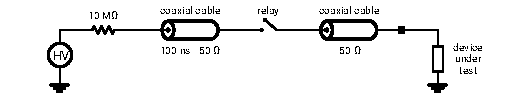
\includegraphics[width=\textwidth]{src/1/figures/tlp_concept.pdf}
  \caption{Minimal example of a \gls{tlp} system}
  \label{tlp_concept}
\end{figure}

% Characteristics of tlp systems
Un système TLP produit des impulsions très reproductibles, car l'environnement est très bien maitrisé et la décharge a lieu dans un chemin de propagation blindé et isolé des perturbations extérieures.
L'impédance characteristique de 50\textOmega{} peut être maintenue jusqu'à la charge The characteristic impedance of  can be controlled up to the load, by using appropriate 50\textOmega{} cables and hardware.
Les propriétés clés d'une impulsion TLP sont données dans la figure \ref{tlp_pulse}.

\begin{figure}[!h]
  \centering
  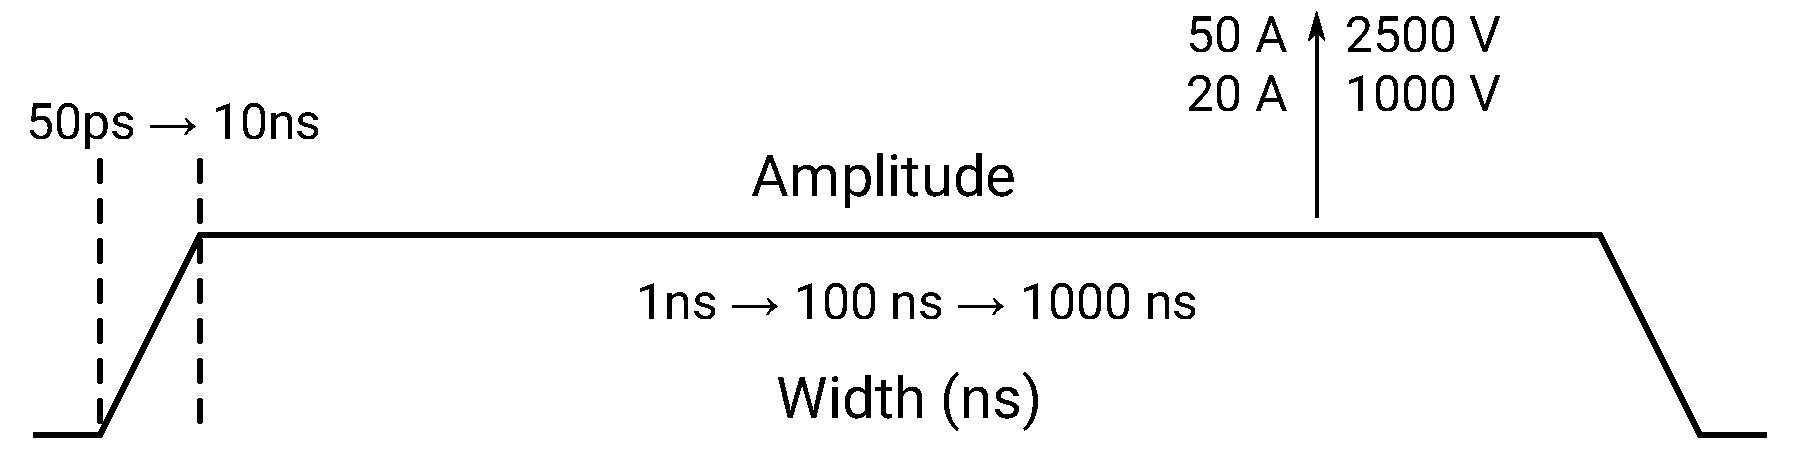
\includegraphics[width=\textwidth]{src/1/figures/tlp_pulse.pdf}
  \caption{Main characteristics of a \gls{tlp} pulse on a resistive load}
  \label{tlp_pulse}
\end{figure}

% ESD guns
Le TLP est un excellent outil de test et d'investigation, mais la forme d'onde est très différente d'une vraie décharge électrostatique.
Pour garantir la robustesse d'un produit, les pistolets de décharge ESD sont préférables.
Les standard IEC 61000-4-2 \cite{iec61000-4-2} et ISO 10605 \cite{iso10605} definissent une forme d'onde de test pour les systèmes électroniques.
Elle reproduit la décharge d'un corps humain à traver un circuit électronique.

Ces tests sont utilisés très largement pour la qualification des produits.
Un pistolet ESD est constitué d'une pointe métallique qui sert à injecter la décharge.
Le retour de masse est assuré par un cable métallique long de quelques mètres.

% How is the pulse generated
La génération de la décharge est assurée en théorie par une résistance de 330\textOmega{} et une capacité de 150.
En pratique, ce réseau RC n'est pas suffisant et les éléments parasites jouent un rôle important.
Le modèle de Chiu \cite{phd-chiu} définit un circuit équivalent de pistolet ESD.
Il est fournit dans la figure \ref{fig:esd-gun-model}.
Un réseau R\textsubscript{g}L\textsubscript{g}C\textsubscript{g} modélise le retour de masse.
Une capacité parasite C\textsubscript{i} ainsi qu'une inductance en série L\textsubscript{i} représentent les imperfections du chemin d'injection.

\begin{figure}[!h]
  \centering
  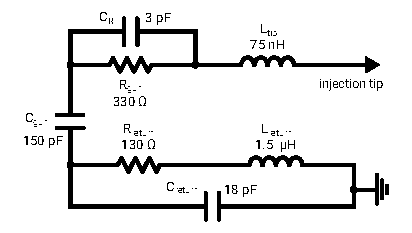
\includegraphics[width=0.3\textwidth]{src/1/figures/gun_model.pdf}
  \caption{ESD Gun model}
  \label{fig:esd-gun-model}
\end{figure}

% Explain the waveform
La forme d'onde est fournie dans la figure \ref{iec_pulse}.
Elle est définie pour une charge de 2\textOmega{}.
L'impulsion commence par un pic d'une largeur de $1ns$ risetime.
Il est suivi par une partie plus lente d'amplitude plus faible, mais qui dure plus longtemps (approximativement $200ns$).
Les niveaux de tensions peuvent atteindre 15kV et de courant 30A.

\begin{figure}[!h]
  \centering
  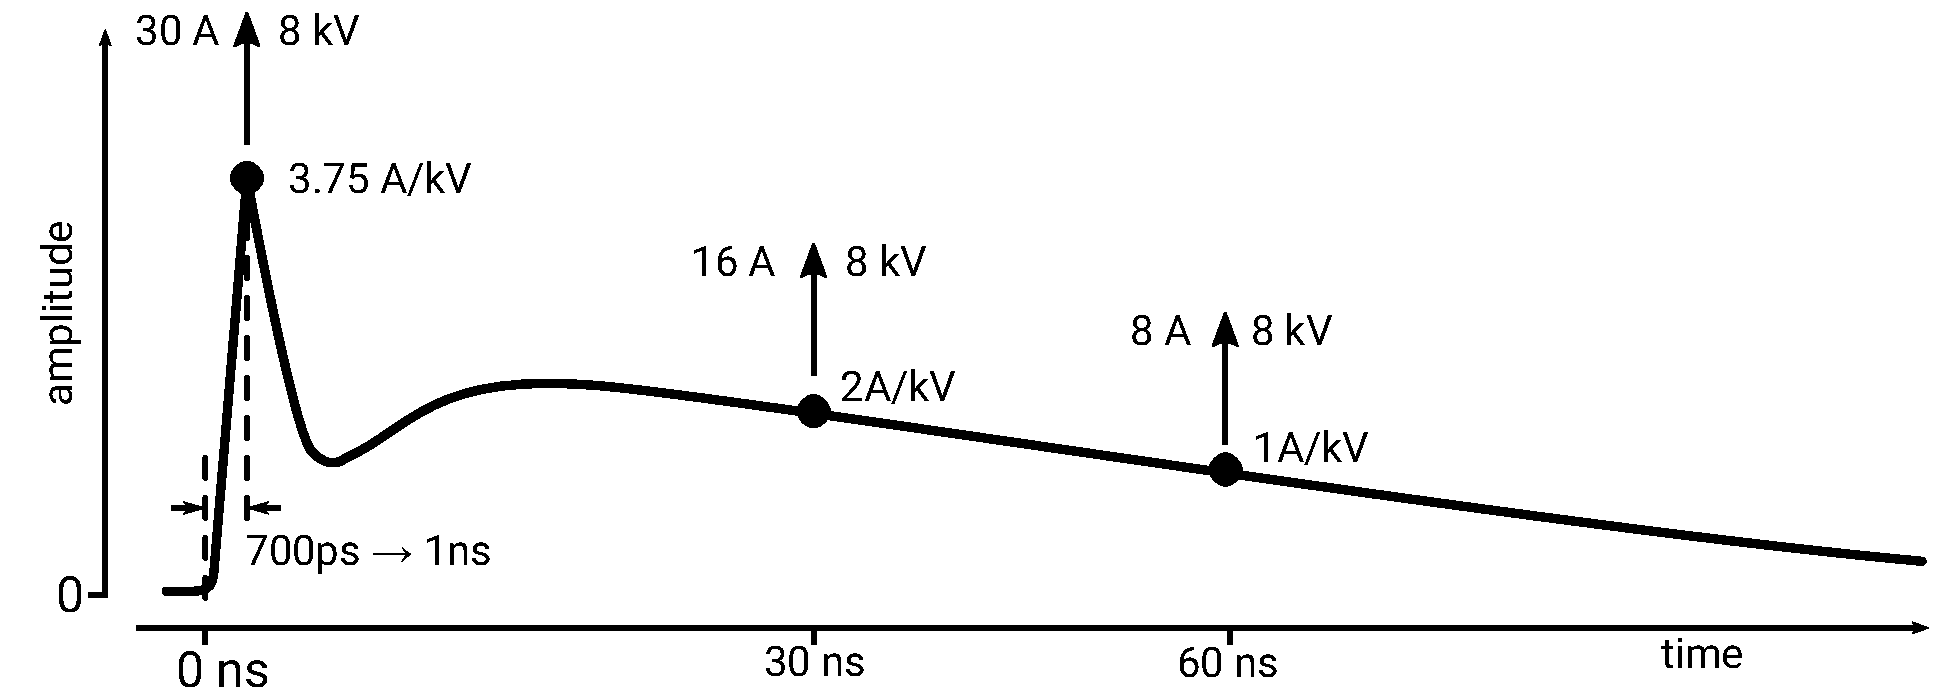
\includegraphics[width=\textwidth]{src/1/figures/iec61000-4-2_waveform.pdf}
  \caption{Main properties of an IEC 61000-4-2 pulse on a 2\textOmega\ resistive load}
  \label{iec_pulse}
\end{figure}

% autres méthodes
Il existe un grand nombre d'autres méthodes de test.
Dans l'automobile, le standard ISO 7637-2 est très largement employée pour qualifier les modules électroniques.
La méthode DPI (Direct Power Injection) est aussi très intéressante de par son circuit de couplage d'un stress sur une tension d'alimentation, ce qui est souvent nécessaire pour faire des tests ESD sur des produits en fonctionnement.

Une fois les produits testés, des cas de défaillances peuvent-être identifiés.
La partie suivante présente des cas de défaillances fonctionnelles trouvés dans la litterature.

\section{Méthodes d'analyse de faiblesses fonctionnelles}

%TODO
% Case 1 - NXP bandgap + substrate coupling
Une sac d'étude typique de défaillance fonctionnelle est présenté par K. Abouda dans \cite{softfailEMCIC}.
L'étude concerne la perte de la régulation de tension assurée normalement dans un circuit intégré pour l'automobile.
La perte de régulation se produit lors d'une exposition du circuit à une décharge BCI (Bulk Current Injection) ISO11452-4 \cite{iso11452}.
Les chemins de propagation et de couplages à l'intérieur du circuit sont recherchés manuellement dans le design du produit, à l'aide de multiples simulations.
Il est démontré qu'un résidu de la décharge modifiait la tension de commande d'un miroir de courant dans une référence bandgap.
Ce résidu atteignait le point perturbé du miroir via un couplage parasite.
A cause de cette perturbation, la tension bandgap chutait de sa tension nominale, au point d'atteindre un seuil bas détecté comme une faute par le système.
En conséquence, le système effectuait un redémarrage complet.
Pour éviter cela, le design a été corrigé afin d'appliquer un filtrage dans le miroir de courant pour éliminer ce résidu.

% Case 2 - CESAME IC - paper Vrignon + Ben dhia
N. Lacrampe présente un autre cas de défaillance dans \cite{LacrampeTransientImmunity}.
Des impulsions Very-fast TLP sont injectées sur un circuit intégré de test en technologie CMOS 0.18 \textmu{}m (1.8 V alimentation).
La puce contient 6 instances du même coeur logique, qui diffèrent par l'architecture de leurs rails d'alimentation.
L'injection sur les rails d'alimentation est effectuée à travers une capacité de 1 nF permet d'isoler le générateur de test de l'alimentation DC.
Cette approche avec une capacité d'injection est similaire au standard DPI \cite{iec62132-4}.
% What is the failure signature
Pour détecter des défaillances, un signal de sortie de la logique est surveillé.
Le critère de susceptibilité est une variation d'amplitude en dessous d'un seuil situé à 80\% du niveau logique haut.
En dessous de ce seuil, les marges de bruit ne permettent plus de garantir un fonctionnement correct du coeur de circuit.
Il est démontré dans ce papier que modéliser le buffer de sortie de la logique est suffisant pour reproduire les formes d'ondes, avec une erreur inférieure à 20\%.
Par conséquent, cette méthode est moins précise qu'une simulation de la schématique entière, mais présente l'avantage d'être plus rapide à simuler.
Les outils de simulation employés dans cette étude sont principalement du VHDL-AMS et des simulations SPICE.

% Case 3 - failures on an SDRAM
Dans \cite{SDRAMCase}, des fautes fonctionnelles sont étudiées sur une mémoire de type SDRAM pendant son fonctionnement normal.
Le système d'injection utilise une cellule TEM (Transverse Electro Magnetic) modifiée de dimensions réduites \ref{fig:modified-tem-cell}, afin d'obtenir des champs électromagnétiques plus forts correspondants à une décharge de pistolet ESD.
La décharge injectée dans la cellule TEM est générée par une impulsion TLP filtrée afin de ressembler à une décharge IEC 61000-4-2 \cite{iec61000-4-2}.
La puce contenant la SDRAM est assemblée sur une carte électronique.
Afin de détecter des fautes, des données sont écrites puis lues en permanence par un FPGA (Field Programmable Gate Array).
Une différence de lecture est alors interprétée comme une défaillance.
Seulement la mémoire est exposée à la perturbation en étant placées à l'intérieur de la cellule TEM.
Le reste des composants de la carte sont localisés de l'autre côté de la carte, à l'extérieur de la cellule.

\begin{figure}[!h]
  \centering
  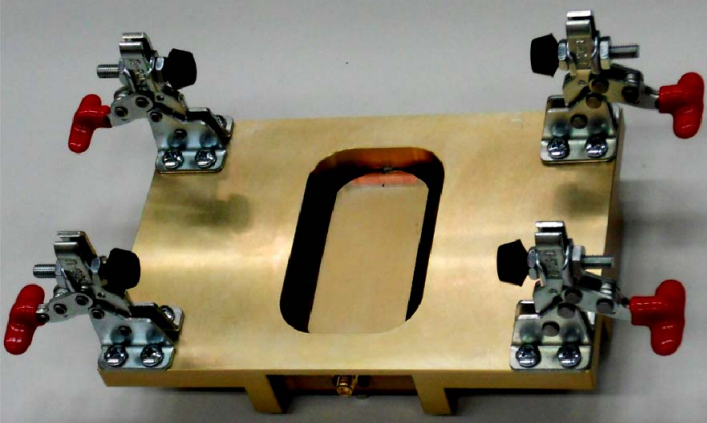
\includegraphics[width=0.6\textwidth]{src/1/figures/modified_tem_cell.png}
  \caption{Modified TEM cell from \cite{SDRAMCase}}
  \label{fig:modified-tem-cell}
\end{figure}

Deux types de défaillances de bus de communication vidéo sont présentés dans \cite{softFailSubsystem}.
En fonction des paramètres de décharge, différents évènements sont observés.
L'objectif de cette étude est de déterminer qui du capteur ou du processeur d'application est responsable de la défaillance.
Une carte d'émission magnétique est enregistrée avec un scanner de champ proche afin d'essayer de détecter des variations locales.
L'hypothèse était qu'une perte de fonctionnalité peut induire des variations significantes sur la carte d'émission, ce qui permettrait de les détecter.
Néanmoins, l'origine des défaillances n'a pas pu être localisé avec cette méthode dans cette étude.

Un affichage LCD (Liquid Crystal Display) est étudié dans \cite{softFailLCD}.
Il est testé à l'aide d'une décharge IEC 61000-4-2 \cite{iec61000-4-2} et des fautes fonctionnelles sont observées.
Des bandes noires apparaissent à la suite de la décharge, ainsi que des variations de paramètres optiques et de rétro-éclairage.
La forme d'onde trop complexe empêchait d'identifier la cause de défaillance, et une solution alternative a du être utilisée.
Une injection par champ proche fut employée afin d'identifier quelle piste du connecteur LCD flex présentait la plus forte susceptibilité.
Néanmoins, les dimensions trop petites du connecteur et des pistes rendaient impossible d'agresser individuellement chaque piste.
Comme alternative, l'utilisation d'un TLP couplé capacitivement sur chaque piste permit une agression individuelle.
Néanmoins, les résultats furent infructueux et aucune piste ne put être identifiée comme point d'entrée de la décharge.

Une méthode d'investigation basée sur des simulations électromagnetiques est présentée dans \cite{softFailMobile} afin de déterminer les chemins de propagation de décharges, causant des fautes sur un appareil mobile.
La décharge de test est celle définie dans IEC 61000-4-2.
Des simulations électromagnetiques temporelles en 3D du téléphone complet furent effectuées (Fig. \ref{fig:mobile-phone-3d-em})
Une fois la cause défaillance déterminée, des réseaux de filtrage RC furent utilisés pour protéger les entrées et sorties physiques telles que les boutons et connecteurs.

\begin{figure}[!h]
  \centering
  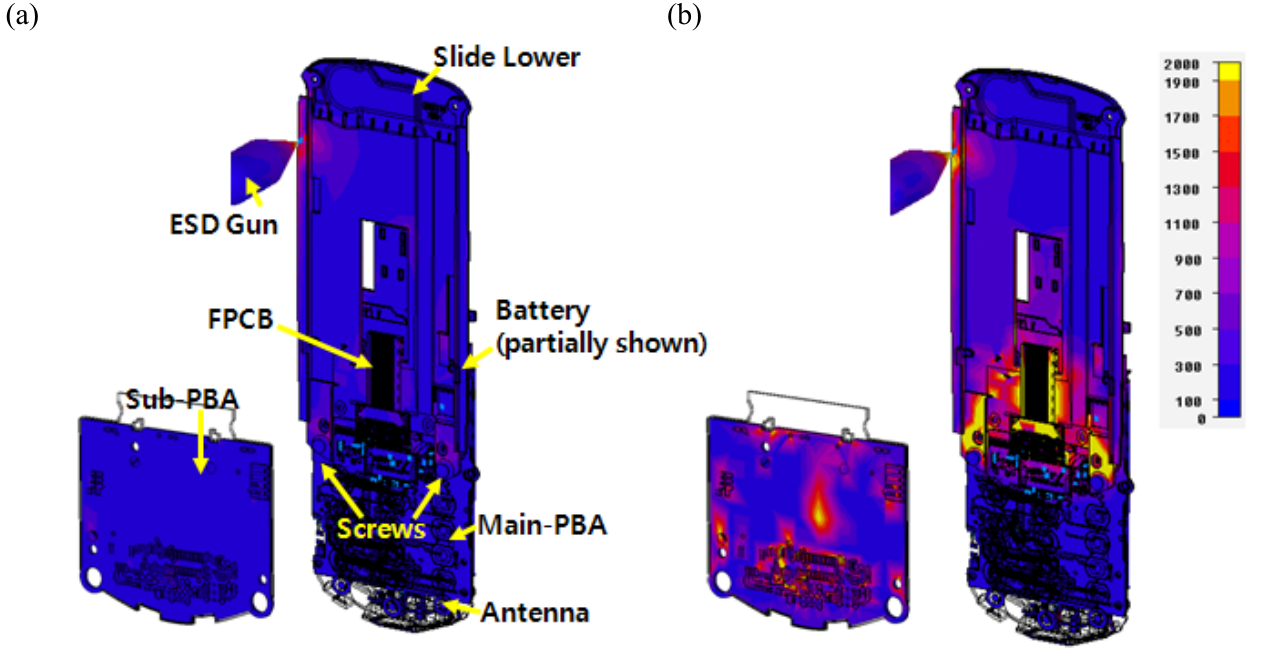
\includegraphics[width=0.8\textwidth]{src/1/figures/current_distribution_mobile.png}
  \caption{ESD Current Distribution on Mobile Phone and Backside sub-battery pack at (a) 1.0 ns and (b) 1.8 ns (Credit: \cite{softFailMobile})}
  \label{fig:mobile-phone-3d-em}
\end{figure}


Near-field scan

% Introduce near-field scanner
Electromagnetic near-field scanner measure maps of electric and magnetic field.
An electric or magnetic probe is swept closely above a device to record the emitted field in near-field conditions.
Measurements may be carried out in the frequency domain or in the time domain.
This tool was initially intended for architectural analysis such as floor-planning and power distribution analysis.
For ESD, spatial information provided by the recorded map is very useful to locate failures and malfunctions.
A comprehensive and detailed analysis of near-field antennas is done by A.D. Yaghjian in \cite{nfsFirstStudy}.
More recent work details the principle of operation, data processing and hardware requirements in \cite{near-field-scan, planarNFSAntenna, NFSMeasurements, NFScanner}.
Finally, measurement of electromagnetic emissions with surface scan method is standardized in IEC TS 61967-3 \cite{iec61967}.
The architecture of a near-field scanner is given in Fig. \ref{fig:near-field-scanner}.

\begin{figure}[!h]
  \centering
  \includegraphics[width=0.4\textwidth]{src/1/figures/architecture_near_field_scanner.pdf}
  \caption{Architecture of a near-field scanning testbench}
  \label{fig:near-field-scanner}
\end{figure}

\begin{figure}[!h]
  \centering
  \includegraphics[width=0.4\textwidth]{src/1/figures/near_field_scanner_susceptibility_map.pdf}
  \caption{Susceptibility map of a board recorded with surface scan in injection configuration \cite{}}
  \label{fig:near-field-scan-map}
\end{figure}

Revue des méthodes de modélisation

In the litterature, various ESD modelling methods can be found.
They comprise a wide range of techniques such as 3D electromagnetic and semiconductor physics simulations, compact, behavioral, physically-based and non-linear modelling.
The methods described hereafter could be used for soft-failure investigation.

M. Scholz details a mixed-mode ESD simulation approach in \cite{mixedModeESDSims}.
It is a combination of \gls{spice} and \gls{tcad} models, simulated in \gls{spice} environment.
The author indicates that the combination of physical device models and standard simulations provides higher accuracy and more realistic simulations than behavioral \gls{spice} models.
Using this complex simulation tool, on-chip and off-chip device interactions are studied, in powered and unpowered conditions.

In \cite{usb2ESDProtection}, TLP characterizations serves as an I(V) model for both external protections and an \gls{ic} pin.
The \gls{pcb} S-parameters are extracted from the board layout, using Momentum software (Agilent Technology).
It is electrically model with lumped R,L,C,G elements.
The modelling approach proved successful for simulation interactions between external devices and on-chip structures.
This method is interesting for soft-failure analysis because it is thorough and complete and enables accurate ESD simulation.

% IBIS is not enough for modelling an IC pin for ESD simulations
The Input Output Buffer Information Specification (IBIS) \cite{ibis-spec} is a behavioral, black-box model for performing signal integrity simulation on digital circuits.
It is widespread in the digital \gls{asic} world because it enables accurate simulations without disclosing circuit or process information.
It was envisionned that IBIS models could also be used or extended for ESD.
It is demonstrated in \cite{ibisImprovementFabrice} that the model lacks some parameters for EMC and ESD simulations.
It comprises a current versus voltage characteristic of \gls{io}s, similar to what can be extracted by a TLP, however the IBIS model is not defined for fast impulses and high injection.

N. Lacrampe proposes in \cite{LacrampeTransientImmunity} to perform 3D electromagnetic simulations at silicon level, using the integrated circuit layout, to deduce the amount of capacitive couplings between Vdd and Vss rails.
The extraction is performed with HFSS software (Ansoft).
The goal of this analysis is to predict the susceptibility of integrated circuits against electrostatic discharges.
\gls{pcb} tracks are modeled by a distributed RLC network.
The package data from the IBIS model \cite{ibis-spec} was used in the simulations.
Finally, a TLP stress generator is modelled using a lookup table I(V) component, in series with a 50\textOmega{} resistor.

Once again, electromagnetic fullwave simulations are conducted in powered-on ESD analysis in \cite{softFailMobile}.
System-level components are simulated, such as PCB, metallic casing and battery back.
3D EM simulations helps to identify the main discharge paths and locate the failure.
